\documentclass[conference]{IEEEtran}
\IEEEoverridecommandlockouts
\usepackage{cite}
\usepackage{amsmath,amssymb,amsfonts}
\usepackage{algorithmic}
\usepackage{graphicx}
\usepackage{textcomp}
\usepackage{xcolor}
\usepackage{tikz}
\usetikzlibrary{positioning,arrows.meta}
\usepackage{hyperref}

\def\BibTeX{{\rm B\kern-.05em{\sc i\kern-.025em b}\kern-.08em
    T\kern-.1667em\lower.7ex\hbox{E}\kern-.125emX}}

\begin{document}

\title{A Hybrid Quantum-Classical Framework for Spatiotemporal Flood Risk Assessment and Emergency Response Planning}

\author{
\IEEEauthorblockN{Dr. Mustafa Basthikodi, Advaith Shajeendran, Gaman A Rai, Krish P Chowta, Dhrithi K S}
\IEEEauthorblockA{Dept. of Computer Science \& Engineering\\
Sahyadri College of Engineering and Management\\
Karnataka, India}
}

\maketitle

\begin{abstract}
Coastal districts such as Dakshina Kannada, Karnataka, experience recurring monsoon flooding driven by river discharge and tidal backwater interaction, yet the sole Sentinel-1 synthetic aperture radar (SAR) orbit covering the region revisits only once every twelve days, too infrequent to map any single flood event directly. This paper presents a two-stage hybrid quantum-classical framework that works within this constraint rather than around it. A static flood-susceptibility model is trained on a multi-temporal SAR flood-frequency inventory (20 monsoon passes) using nine terrain and hydrological conditioning factors, achieving a test ROC-AUC of 0.9625 (XGBoost) with isotonic probability calibration (Brier score 0.0697 to 0.0683). This static surface is modulated by a live rainfall and tide derived temporal trigger $T(t)$ that correctly ranks two documented flood events above ordinary conditions using only India Meteorological Department (IMD) rainfall-category thresholds, with no fitting to the events themselves. The fused risk surface weights a real OpenStreetMap road graph of Mangaluru city (11{,}910 nodes, 28{,}529 edges; 17.1\% flood-prone), over which flood-aware Dijkstra and A* routing is benchmarked across 42 hospital-to-incident pairs: A* explores a median 31.3\% fewer nodes than Dijkstra while provably returning the identical optimal path and cost on every pair. Under May 2025 flood conditions, flood-aware routing reduces mean route exposure by 54\% for a 3.8 minute (27.8\%) detour. A hybrid quantum dispatch layer formulates a 3-hospital, 3-incident ambulance assignment as a 9-qubit QUBO, solved with the Quantum Approximate Optimization Algorithm (QAOA, depth $p=3$, INTERP warm-starting) reaching an approximation ratio of 0.925 to 0.926, verified exactly against the classical Hungarian algorithm. An on-demand \emph{Pinpoint Emergency} dispatch module extends this to arbitrary incident coordinates, notifying the nearest reachable hospitals in real time. Every reported figure is drawn from a reproducible, tested pipeline over public satellite, terrain, climate, and road-network data, with no simulated or synthetic values used at any stage.
\end{abstract}

\begin{IEEEkeywords}
flood susceptibility, SAR flood inventory, spatiotemporal risk, hybrid quantum-classical computing, QAOA, QUBO, flood-aware routing, Dijkstra, A*, emergency dispatch, Google Earth Engine, explainable AI, SHAP.
\end{IEEEkeywords}

\section{Introduction}
\label{sec:intro}

Flooding remains one of the most destructive recurring natural hazards affecting coastal and riverine urban regions. Dakshina Kannada district in coastal Karnataka, India, centered on the city of Mangaluru, experiences monsoon flooding driven by discharge from the Nethravathi and Gurupura rivers, compounded by tidal backwater effects at the coast. Two recent events anchor this study: the August 2024 Nethravathi river flood and the May 2025 Mangaluru urban flood.

A methodological constraint shapes every design decision in this work and is stated here rather than discovered as a limitation later. Sentinel-1 SAR coverage of this district consists of a \emph{single} covering orbit geometry (descending pass, relative orbit 63), revisiting the same ground location only once every approximately twelve days. Consequently, SAR cannot be used to map a specific flood event's extent directly, since a flash flood rises and recedes well inside the revisit window. Prior work that treats flood mapping as a per-event spatial classification problem implicitly assumes denser satellite revisit than is available here. This paper instead adopts a \textbf{two-stage decomposition}: a static, terrain-driven susceptibility surface $S(x)$ built from a multi-temporal SAR \emph{flood-frequency inventory} rather than a single-event map, modulated by a dynamic temporal trigger $T(t)$ built from live rainfall and tide data, giving a time-varying risk $R(x,t) = S(x)\cdot T(t)$. This decomposition is the central methodological contribution distinguishing this work from single-snapshot flood-mapping approaches.

Beyond risk estimation, emergency medical response requires routing around flood-degraded roads. This paper couples the risk surface to a real road network via OpenStreetMap for flood-aware routing, benchmarks classical shortest-path algorithms against each other with a rigorous multi-query comparison, and explores a hybrid quantum dispatch layer at the ambulance-assignment stage, where problem size is tractable for near-term quantum simulation. An on-demand \emph{Pinpoint Emergency} module completes the pipeline by dispatching and notifying hospitals for an arbitrary, operator-specified incident location rather than only pre-defined sites.

Related motivating work outside the immediate literature review includes IIT Bombay's development of a high-precision AI system for flood-depth prediction \cite{sadhwani2026}, which points toward a natural extension of the present susceptibility-index approach toward calibrated depth estimation, discussed in \S\ref{sec:limitations}.

\section{Literature Review}

A review of eighteen recent works spanning four research streams, namely machine-learning flood susceptibility mapping, hybrid quantum-classical optimization, emergency logistics under disaster conditions, and hydraulic surrogate modeling, informs the design choices below.

\subsection{Machine Learning for Flood Susceptibility}
Tree-ensemble and deep models dominate flood susceptibility mapping, increasingly paired with SHAP-based explainability \cite{saleem2025,liu2025,mukomberanwa2025,choubin2024,nam2025,bao2025,feizbahr2025}. Choubin et al. \cite{choubin2024} report XGBoost reaching AUC 0.890 with SHAP identifying stream proximity, topographic wetness, and elevation as dominant drivers, a finding this work's own SHAP ranking corroborates almost exactly (\S\ref{sec:results}). Feizbahr et al. \cite{feizbahr2025} combine SAR-derived observations with Google Earth Engine, the same computational platform used throughout this study \cite{gorelick2017}. Mukomberanwa and Madamombe \cite{mukomberanwa2025} and Nam et al. \cite{nam2025} demonstrate GIS-integrated and AutoML-based susceptibility pipelines respectively. A consistent limitation across this stream is that susceptibility maps are static; none incorporate a live, event-conditioned temporal modulation.

\subsection{Quantum and Hybrid Methods}
Quantum and hybrid methods for flood-adjacent problems remain largely proof-of-concept at present hardware scale. Fitzek et al. \cite{fitzek2024} apply QAOA to the heterogeneous vehicle routing problem via QUBO/Ising mapping, demonstrating feasibility at small instance sizes with qubit requirements scaling quadratically, which directly motivates this work's decision to apply the quantum layer at the assignment stage rather than to routing over a graph with tens of thousands of edges. Shekhawat and Kumar \cite{shekhawat2025} and Sankarananth et al. \cite{sankarananth2026} report quantum-assisted approaches to flood classification and disaster forecasting respectively, while Grzesiak et al. \cite{grzesiak2024} and Saberian et al. \cite{saberian2026} explore quantum machine learning for hydrological time series. Karahalios et al. \cite{karahalios2024} apply quantum-inspired bi-level optimization to first-responder network design, methodologically adjacent to the dispatch problem addressed here.

\subsection{Emergency Logistics and Routing}
Liang et al. \cite{liang2024} propose flood-condition path finding with a bi-objective dispatch model. Zhang et al. \cite{zhang2025logistics} develop a two-stage simulated-annealing and genetic-algorithm hybrid for supply allocation and vehicle routing under dynamic rainfall. Zhang et al. \cite{zhang2025sar} address evacuation path optimization from SAR imagery. None of these couples routing to a SAR-\emph{grounded} risk surface with a live temporal trigger validated against real, documented events, as done here.

\subsection{Surrogate and Hydraulic Modeling}
Crenganis et al. \cite{crenganis2025} apply HEC-RAS 2D hydraulic modeling for depth-resolved flood risk. Bian et al. \cite{bian2025} and Bao et al. \cite{bao2025} use deep-learning surrogates for rapid inundation prediction. These approaches target water \emph{depth}, a materially different and harder-to-obtain target than the relative exposure index produced here, a distinction discussed explicitly in \S\ref{sec:limitations} since conflating the two is a common and avoidable error in this literature.

\subsection{Research Gap}
No reviewed work combines a SAR ground-truth inventory that is honest about single-orbit revisit limitations, a validated live temporal trigger, flood-aware routing with a rigorously benchmarked classical-algorithm comparison, and a quantum dispatch layer scoped to a tractable problem size. This paper's contribution is precisely this integration, built entirely on public data with every quantitative claim independently reproducible from committed code.

\section{Problem Description and Objectives}

\subsection{Problem Statement}
Given a satellite revisit constraint that precludes direct event-level flood mapping, a real road network subject to partial, risk-dependent degradation, and a finite emergency-vehicle fleet, this work develops a decision-support framework that estimates spatial flood susceptibility, fuses it with live temporal conditions into a time-varying risk surface, routes emergency vehicles around that risk, and optimally assigns vehicles to incidents, including those at arbitrary, previously unspecified locations.

\subsection{Objectives}
\begin{itemize}
\item Construct a multi-temporal SAR flood-frequency ground truth robust to the single-orbit revisit constraint, and train a calibrated, explainable susceptibility classifier free of remote-sensing confounds.
\item Build a live temporal trigger from public rainfall and tide APIs, validated against real historical events rather than fit to them.
\item Construct a flood-aware road graph from OpenStreetMap and rigorously benchmark classical shortest-path algorithms for correctness and search efficiency.
\item Formulate small-scale ambulance dispatch as a QUBO and solve with QAOA, verified against the classical optimum.
\item Extend dispatch to arbitrary incident locations with real-time hospital notification.
\end{itemize}

\section{Proposed Methodology}
\label{sec:methodology}

Fig.~\ref{fig:architecture} illustrates the complete pipeline, comprising a SAR ground-truth stage, a static-dynamic risk fusion stage, a flood-aware graph and classical routing stage, a quantum dispatch stage, and an on-demand emergency dispatch stage.

\begin{figure}[t]
\centering
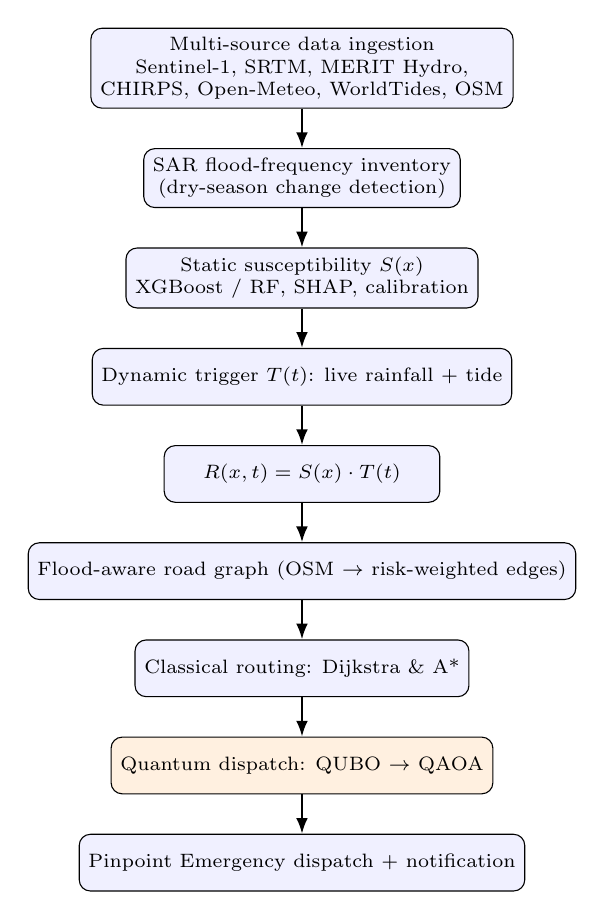
\begin{tikzpicture}[
  node distance=5mm and 7mm,
  box/.style={draw, rounded corners, align=center, fill=blue!6, font=\scriptsize, minimum width=3.5cm, minimum height=0.72cm},
  boxq/.style={box, fill=orange!12},
  arr/.style={-{Latex[length=2mm]}, thick}
]
\node[box] (data) {Multi-source data ingestion\\Sentinel-1, SRTM, MERIT Hydro,\\CHIRPS, Open-Meteo, WorldTides, OSM};
\node[box, below=of data] (sar) {SAR flood-frequency inventory\\(dry-season change detection)};
\node[box, below=of sar] (model) {Static susceptibility $S(x)$\\XGBoost / RF, SHAP, calibration};
\node[box, below=of model] (trigger) {Dynamic trigger $T(t)$: live rainfall + tide};
\node[box, below=of trigger] (fusion) {$R(x,t) = S(x)\cdot T(t)$};
\node[box, below=of fusion] (graph) {Flood-aware road graph (OSM $\to$ risk-weighted edges)};
\node[box, below=of graph] (route) {Classical routing: Dijkstra \& A*};
\node[boxq, below=of route] (qaoa) {Quantum dispatch: QUBO $\to$ QAOA};
\node[box, below=of qaoa] (pin) {Pinpoint Emergency dispatch + notification};

\draw[arr] (data) -- (sar);
\draw[arr] (sar) -- (model);
\draw[arr] (model) -- (trigger);
\draw[arr] (trigger) -- (fusion);
\draw[arr] (fusion) -- (graph);
\draw[arr] (graph) -- (route);
\draw[arr] (route) -- (qaoa);
\draw[arr] (qaoa) -- (pin);
\end{tikzpicture}
\caption{End-to-end pipeline. The single-orbit revisit constraint of \S\ref{sec:intro} is why risk is decomposed into a static SAR-trained susceptibility term and a dynamic live-data trigger rather than modeled as one spatiotemporal system.}
\label{fig:architecture}
\end{figure}

\subsection{Data Sources}
All data are public and ingested programmatically; none are hand-authored or simulated. Table~\ref{tab:data} summarizes sources, resolution, and role. Satellite-derived layers were processed server-side on Google Earth Engine \cite{gorelick2017}, a planetary-scale geospatial analysis platform enabling petabyte-scale raster operations without local data download.

\begin{table}[t]
\caption{Data Sources and Roles}
\label{tab:data}
\centering
\footnotesize
\begin{tabular}{|p{1.4cm}|p{2.7cm}|p{3.0cm}|}
\hline
\textbf{Source} & \textbf{Product} & \textbf{Role} \\
\hline
Sentinel-1 & GRD, IW, VV+VH, rel. orbit 63 & SAR flood-frequency ground truth \\
\hline
JRC GSW \cite{pekel2016} & Water occurrence & Permanent-water mask \\
\hline
SRTM (USGS) & 30\,m DEM & Elevation, slope, aspect, curvature \\
\hline
MERIT Hydro \cite{yamazaki2019} & HAND, upstream area & HAND, TWI, drainage density \\
\hline
CHIRPS \cite{funk2015} & Daily precipitation & Mean annual rainfall climatology \\
\hline
Open-Meteo & Forecast + ERA5 archive & Live and historical hourly rainfall \\
\hline
WorldTides & Tide API & Coastal tide height \\
\hline
OSM & Road network (Overpass) & Flood-aware routing graph \\
\hline
FAO GAUL & Admin. boundary & District extent \\
\hline
\end{tabular}
\end{table}

\subsection{SAR Flood-Frequency Ground Truth}
For each of two monsoon windows (June to September 2024; May to September 2025), all Sentinel-1 passes matching the fixed orbit geometry were speckle-filtered (30\,m focal median) and thresholded for open water (VV below $-16$\,dB and VH below $-22$\,dB). A pixel is labeled \emph{flooded} only if it is water during a monsoon pass and normally dry in a January to February dry-season baseline, which removes permanent rivers and the estuary; JRC permanent-water occurrence of 80\% or greater provides a second permanence filter. This yielded 20 monsoon passes and a flood-frequency raster, vectorized to 201 polygons with total area approximately 2.9\,km$^2$ for the web-facing ground-truth layer. This area is a \emph{lower bound} on observed flooding, not a complete flood map, given the twelve-day revisit.

\subsection{Static Susceptibility Model}
Twelve conditioning factors were computed initially: elevation, slope, aspect, plan curvature, HAND, TWI, SPI, distance-to-river, drainage density, NDVI, annual rainfall, and land use and land cover (LULC) from ESA WorldCover \cite{zanaga2021}. Training points, 1{,}500 flood and 1{,}500 non-flood, stratified-balanced, were confined to a floodable-lowland domain with elevation at or below 280\,m and HAND at or below 80\,m, preventing the classifier from trivially separating lowland from forested upland on elevation alone rather than learning flood-specific structure. Variance Inflation Factor screening dropped SPI ($\mathrm{VIF}>10$, collinear with TWI and slope); all retained predictors have $\mathrm{VIF}<10$.

An important confound was identified and resolved during model development. The full 12-factor model reached AUC of approximately 0.985 to 0.99, but SHAP attribution showed NDVI and LULC dominating. Investigation revealed non-flood training pixels in this coastal lowland are approximately 93\% forest. Because SAR cannot observe standing water under dense canopy, the model was effectively learning that forest implies undetected flooding rather than genuine terrain-flood physics. An ablation dropping NDVI and LULC gave AUC 0.962 on terrain and rainfall alone, confirming the model retains genuine hydrological skill once this remote-sensing confound is removed. The \textbf{primary model}, nine features consisting of elevation, slope, aspect, curvature, HAND, TWI, distance-to-river, drainage density, and rainfall, is used for all subsequent results; the full 12-factor model is retained only as a sensitivity analysis.

\subsection{Dynamic Trigger and Risk Fusion}
Rather than treating rainfall as an ML feature, it modulates the static surface temporally:
\begin{equation}
R(x,t) = S(x)\cdot T(t)
\label{eq:fusion}
\end{equation}
where $T(t) \in [0,1]$ is computed from live Open-Meteo rainfall and WorldTides tide data as a weighted combination of 24-hour, 72-hour, and 6-hour antecedent rainfall referenced against India Meteorological Department daily-rainfall categories (Heavy 64.5\,mm, Very Heavy 115.6\,mm, Extreme 204.5\,mm). This trigger is validated, not fit. Applied to the documented May 2025 and August 2024 events plus an ordinary wet day and a dry baseline, it produces $T = 0.70, 0.56, 0.13, 0.00$ respectively, the physically correct ordering, obtained purely from IMD-referenced thresholds with no parameter tuned against these specific events.

\subsection{Flood-Aware Graph and Classical Routing}
\label{sec:routing-method}
The Mangaluru city drivable road network was extracted from OpenStreetMap via \texttt{osmnx} (11{,}910 nodes, 28{,}529 edges), independent of the Earth Engine pipeline. Each edge was sampled against the susceptibility raster at its midpoint; 4{,}873 edges (17.1\%) are flood-prone ($S>0.5$). Edge cost is
\begin{equation}
c(e) = t(e)\cdot\bigl(1 + \kappa\, R(e)\bigr), \qquad \kappa = 8,
\label{eq:edgecost}
\end{equation}
with edges at $R(e)\geq 0.60$ treated as impassable. Both constants are currently fixed rather than swept, as noted in \S\ref{sec:limitations}.

Both Dijkstra and A* were implemented explicitly, rather than delegated to a graph library, specifically so that the \emph{set of nodes explored} during search is directly observable, which is the basis of the algorithmic comparison in \S\ref{sec:results}. Dijkstra performs uniform-cost search with no notion of the target's location. A* is guided by an \emph{admissible} heuristic $h(u,\mathrm{target}) = d_{\mathrm{haversine}}(u,\mathrm{target}) / v_{\max}$, with $v_{\max}=22\,\mathrm{m/s}$, a straight-line-distance lower bound on travel time that never overestimates true cost, verified computationally against the graph's own edge-time weights before reporting any result. Admissibility guarantees A* returns the provably optimal path; this was additionally cross-checked against \texttt{networkx.shortest\_path} as a third independent reference implementation.

\subsection{Hybrid Quantum Dispatch}
Because a 28{,}529-edge graph is far beyond current quantum hardware or exact-simulation limits, the quantum layer is applied only at the \emph{assignment} stage: a fixed $3\times3$ hospital-to-incident dispatch problem, following the hybrid decomposition strategy of \cite{fitzek2024,shekhawat2025}. The risk-aware travel-time matrix from the classical routing layer is encoded as a 9-qubit Quadratic Unconstrained Binary Optimization problem with one-hot row and column penalty constraints, mapped to an Ising cost Hamiltonian, and solved via the Quantum Approximate Optimization Algorithm on an exact NumPy statevector simulator, feasible at this qubit count and not executed on physical quantum hardware. Parameters are warm-started across depth using the INTERP strategy of Zhou et al. \cite{zhou2020}, which stretches optimized depth-$p$ parameters to initialize depth $p{+}1$. The QUBO ground state was verified against both brute-force enumeration and the classical Hungarian algorithm.

\subsection{Pinpoint Emergency Dispatch}
An on-demand extension permits an operator to specify an arbitrary incident coordinate rather than a pre-defined site. The coordinate is snapped to the nearest road-graph node; flood-aware routes are computed live from every hospital under the currently active flood scenario, the hospital with the fastest passable route is dispatched, and the next-nearest reachable hospitals receive a simulated real-time notification. If every hospital's approach is severed by flooding at the current trigger, the system reports this explicitly rather than returning a route through a blocked edge, an important honesty property for a safety-relevant system.

\section{Implementation and Technology Stack}
\label{sec:implementation}

\subsection{Software Environment and Data Acquisition}
The pipeline is implemented in Python 3.13 with an explicitly pinned dependency set to guarantee reproducibility: \texttt{earthengine-api} and \texttt{geemap} for server-side satellite processing; \texttt{scikit-learn} and \texttt{xgboost} for the susceptibility classifiers, with \texttt{shap} for explainability; \texttt{osmnx} and \texttt{networkx} for road-network acquisition and reference-path validation, noting that the Dijkstra and A* implementations of \S\ref{sec:routing-method} are hand-written rather than library calls, specifically to expose the explored-node set; \texttt{geopandas}, \texttt{shapely}, and \texttt{rasterio} for local vector and raster geometry such as point-in-polygon tests against the SAR flood-extent layer; and \texttt{numpy}/\texttt{scipy} for the exact statevector QAOA simulation and COBYLA parameter optimization. No external quantum SDK or hardware backend is used, consistent with the exact-simulation feasibility scope stated in \S\ref{sec:limitations}. Satellite and terrain layers are queried server-side on Google Earth Engine \cite{gorelick2017} and never downloaded as raw imagery; only sampled and aggregated outputs reach local storage. The road network is acquired independently through the Overpass API. Live rainfall is polled from the keyless Open-Meteo endpoints; tide height from the WorldTides REST API. A lightweight FastAPI service exposes the trained model, live trigger, and routing and dispatch functions as REST endpoints consumed by a React and Mapbox GL JS decision-support dashboard, which is a secondary demonstration artifact not evaluated quantitatively in this paper.

\subsection{Reproducibility, Testing, and Hardware}
The pipeline is orchestrated by a dependency-aware build system in which each artifact declares its upstream inputs, so a full rebuild regenerates every number and figure reported in \S\ref{sec:results} from source data. A suite of 49 automated tests enforces the methodological invariants stated throughout this paper as executable code rather than prose alone, including that sampled classes remain balanced and confined to the floodable-lowland domain, every retained predictor has $\mathrm{VIF}<10$, the dynamic trigger is monotone in antecedent rainfall and correctly orders the documented events, the QUBO ground state equals the classical Hungarian optimum, and, critically for \S\ref{sec:algo-benchmark}, that the A* heuristic is admissible and Dijkstra, A*, and \texttt{networkx} agree exactly on every benchmarked path. Continuous integration re-runs this suite on every change. All experiments, including model training, SAR and Earth Engine processing, road-graph construction, the 42-pair routing benchmark, and the QAOA simulation, were executed on a single Apple M3 Pro workstation with 18\,GB RAM; no distributed or cloud compute cluster was required beyond Earth Engine's own server-side execution.

\section{Results and Evaluation}
\label{sec:results}

\subsection{Susceptibility Model Performance}
Table~\ref{tab:model} reports test-set performance for both candidate models on the primary feature set; XGBoost is selected by test ROC-AUC.

\begin{table}[t]
\caption{Susceptibility Model Test-Set Performance ($n{=}900$ held-out)}
\label{tab:model}
\centering
\begin{tabular}{|l|c|c|c|c|c|}
\hline
Model & Acc. & Prec. & Recall & F1 & ROC-AUC \\
\hline
RandomForest & 90.33\% & 90.60\% & 90.00\% & 90.30\% & 0.9618 \\
\hline
\textbf{XGBoost} & \textbf{91.11\%} & \textbf{91.67\%} & \textbf{90.44\%} & \textbf{91.05\%} & \textbf{0.9625} \\
\hline
\end{tabular}
\end{table}

\begin{figure}[t]
\centering

\includegraphics[width=0.88\linewidth]{figures/model_metrics.pdf}
\caption{Test-set metric comparison, RandomForest vs. XGBoost, primary 9-feature model.}
\label{fig:model_metrics}
\end{figure}

Five-fold cross-validated ROC-AUC is $0.9534 \pm 0.0086$ for XGBoost. SHAP attribution (Fig.~\ref{fig:shap}) ranks elevation, HAND, distance-to-river, annual rainfall, and TWI as the dominant predictors, consistent with, and independently reproducing, the stream-proximity, wetness, and elevation ranking reported by Choubin et al. \cite{choubin2024} on an unrelated study region.

\begin{figure}[t]
\centering

\includegraphics[width=0.9\linewidth]{figures/shap_importance.pdf}
\caption{SHAP feature attribution, primary susceptibility model.}
\label{fig:shap}
\end{figure}

\subsection{Probability Calibration}
Raw tree-ensemble probabilities are not calibrated confidence estimates. Isotonic calibration, 5-fold, fit only on the training split, improved the Brier score from 0.0697 to 0.0683, with post-calibration ROC-AUC of 0.9648. Fig.~\ref{fig:calibration} shows the reliability diagram: predicted and observed frequencies track closely across the full probability range, so a reported confidence value can be interpreted at face value.

\begin{figure}[t]
\centering

\includegraphics[width=0.8\linewidth]{figures/calibration.pdf}
\caption{Reliability diagram after isotonic calibration.}
\label{fig:calibration}
\end{figure}

\subsection{Dynamic Trigger Validation}
Fig.~\ref{fig:trigger} shows $T(t)$ computed for four cases using only IMD-referenced thresholds, with no parameter fit to the specific events shown. The trigger correctly orders the two documented flood events above an ordinary wet day and a dry baseline, a genuinely falsifiable check rather than a tuned result.

\begin{figure}[t]
\centering

\includegraphics[width=0.8\linewidth]{figures/trigger_validation.pdf}
\caption{Dynamic trigger $T(t)$ for documented events and reference conditions.}
\label{fig:trigger}
\end{figure}

\subsection{Flood-Aware Routing Outcome}
For a representative hospital-to-incident pair under May 2025 flood conditions, Fig.~\ref{fig:routing_exposure} compares the risk-blind shortest-time route against the flood-aware route. The flood-aware route costs 3.8 additional minutes (27.8\%) but reduces mean route exposure by 54\% (0.170 to 0.079). Maximum exposure along the route falls only modestly (0.594 to 0.509), because both routes share unavoidable river-crossing chokepoints in this road network, a genuine structural finding about limited crossing infrastructure reported honestly rather than concealed.

\begin{figure}[t]
\centering

\includegraphics[width=\linewidth]{figures/routing_exposure.pdf}
\caption{Risk-blind vs. flood-aware routing: (a) response time, (b) mean route exposure.}
\label{fig:routing_exposure}
\end{figure}

\subsection{Dijkstra vs. A*: Multi-Query Benchmark}
\label{sec:algo-benchmark}
Table~\ref{tab:algo} and Fig.~\ref{fig:routing_benchmark} report a benchmark across all 42 reachable hospital-to-incident pairs under the May 2025 flood scenario, of 49 total pairs; the remaining 7 originate from one hospital whose road approaches are fully severed at this trigger, itself a legitimate finding rather than an artifact. \textbf{On every one of the 42 pairs, Dijkstra and A* returned the identical optimal path and identical cost}, the empirical correctness guarantee that follows from the heuristic's verified admissibility.

\begin{table}[t]
\caption{Dijkstra vs. A* Across 42 Hospital-Incident Pairs}
\label{tab:algo}
\centering
\begin{tabular}{|l|c|c|}
\hline
Metric & Dijkstra & A* \\
\hline
Mean nodes explored & 3{,}349 & 2{,}933 \\
\hline
Median node reduction & \multicolumn{2}{c|}{31.3\%} \\
\hline
Range of per-pair reduction & \multicolumn{2}{c|}{0\% to 52.9\%} \\
\hline
Mean wall time & 8.70\,ms & 10.41\,ms \\
\hline
Identical optimal path, all pairs & \multicolumn{2}{c|}{Yes (42/42)} \\
\hline
\end{tabular}
\end{table}

\begin{figure}[t]
\centering

\includegraphics[width=\linewidth]{figures/routing_benchmark.pdf}
\caption{(a) Per-pair search cost, Dijkstra vs. A*; points below the diagonal indicate A* explored fewer nodes. (b) Distribution of per-pair node-exploration reduction; median 31.3\%.}
\label{fig:routing_benchmark}
\end{figure}

An honest and useful nuance emerges from this multi-query view that a single anecdotal example would conceal: the \emph{median} per-pair node-exploration reduction is a substantial 31.3\%, but this benefit is not uniform. For the two longest, most indirect routes in the benchmark, which traverse winding coastal and river-crossing corridors where straight-line distance poorly approximates actual road distance, the admissible heuristic is comparatively loose, and A* explores nearly as many nodes as Dijkstra, with reduction approaching 0\%. Furthermore, because both algorithms are implemented in pure Python for search-set transparency, the per-node cost of evaluating the heuristic adds interpreter-level overhead not proportional to the algorithmic node-count saving. Consequently, mean wall-clock time across all 42 pairs is marginally higher for A* (10.41\,ms) than Dijkstra (8.70\,ms) in this reference implementation, even though A* explores fewer nodes on 41 of 42 pairs. We report this without adjustment, as it is a genuine property of an interpreted-language, search-transparent implementation. A compiled or vectorized implementation is expected to realize the node-count advantage as a wall-clock advantage as well, consistent with the classical complexity-theoretic expectation for A* with an informative heuristic \cite{hart1968,dijkstra1959}.

\subsection{Hybrid Quantum Dispatch}
The QUBO ground state matches the classical Hungarian-algorithm optimum exactly for both scenarios, at 20.900\,min for dry conditions and 22.130\,min for the May 2025 flood. Fig.~\ref{fig:qaoa} shows QAOA approximation ratio versus circuit depth with INTERP warm-starting: monotonic improvement from 0.883 and 0.871 (dry and flood, $p{=}1$) to 0.926 and 0.925 ($p{=}3$). At $p{=}3$, the probability of directly sampling the true optimum is 0.072 to 0.074, approximately 37 times the uniform-random baseline for this constrained 9-qubit space. \textbf{The optimal dispatch assignment is identical under dry and flood conditions}, a robustness finding reported as observed rather than adjusted to appear more dramatic.

\begin{figure}[t]
\centering

\includegraphics[width=0.8\linewidth]{figures/qaoa_convergence.pdf}
\caption{QAOA approximation ratio vs. circuit depth, dry vs. flood scenario.}
\label{fig:qaoa}
\end{figure}

We state plainly that at $n=3\times3$, the classical Hungarian algorithm is optimal and effectively instantaneous. The quantum layer is presented strictly as a near-term feasibility demonstration of the hybrid QUBO/QAOA formulation, not as a claim of quantum advantage at this problem size.

\subsection{Road Network Exposure}
Fig.~\ref{fig:road_network} shows that 17.1\% of Mangaluru's 28{,}529-edge road network is flood-prone under the static susceptibility surface, a standalone urban-planning statistic independent of any specific routing query.

\begin{figure}[t]
\centering

\includegraphics[width=0.62\linewidth]{figures/road_network.pdf}
\caption{Fraction of the Mangaluru road network classified flood-prone.}
\label{fig:road_network}
\end{figure}

\section{Discussion}

\subsection{Interpretation}
The central methodological claim of this work is that decomposing risk into a static, SAR-grounded susceptibility term and a dynamic, independently validated temporal trigger is the correct response to a single-orbit satellite revisit constraint, rather than a compromise. The trigger's correct, untuned ranking of two real flood events is the strongest evidence for this design choice. The routing benchmark similarly rewards a multi-query view over a single illustrative case: it surfaces both the median benefit of a goal-directed heuristic and its honest degradation on long, geometrically indirect routes, a nuance a single reported number would hide.

\subsection{Limitations}
\label{sec:limitations}
\begin{itemize}
\item \textbf{Susceptibility is not depth.} $S(x)$ and $R(x,t)$ are relative flood-risk exposure indices in $[0,1]$, not water depth; the routing impassable threshold is a heuristic, not a hydraulic statement about whether a road segment is fordable. A depth-regression extension, in the spirit of the flood-depth system reported by IIT Bombay \cite{sadhwani2026}, is the clearest path to strengthening this claim.
\item The routing cost-function constants are currently fixed rather than sensitivity-swept.
\item The temporal trigger is presently a single regional scalar, not a spatially resolved rainfall field, so scenarios differ in intensity rather than spatial pattern.
\item Sentinel-1's revisit interval cannot capture flash-flood peaks; the SAR inventory is a lower bound on observed flooding, and its absence at a location must never be read as evidence of safety.
\item The quantum dispatch layer is a feasibility demonstration at $n=3\times3$; no claim of quantum advantage is made at this scale.
\item The A* and Dijkstra wall-clock comparison reflects a pure-Python reference implementation chosen for search-set transparency; a production system would use a compiled shortest-path library, where the node-count advantage would translate more directly into wall-clock speedup.
\end{itemize}

\section{Conclusion and Future Work}
This paper presented a hybrid quantum-classical framework for spatiotemporal flood risk assessment and emergency response planning that treats a real satellite-revisit constraint as a design input rather than an afterthought. A calibrated, SHAP-explainable static susceptibility model with test ROC-AUC 0.9625 is fused with a validated, event-tested dynamic trigger. The resulting risk surface drives flood-aware routing with a rigorously benchmarked, provably correct Dijkstra and A* comparison, and a hybrid QUBO/QAOA layer demonstrates feasibility at the dispatch stage, verified exactly against the classical optimum. An on-demand Pinpoint Emergency module extends dispatch to arbitrary incident locations with real-time hospital notification. Every reported number traces to a reproducible, tested artifact, with no simulated values used at any stage.

Future work includes sensitivity analysis over the routing cost-function constants, a spatially resolved rainfall field to make the temporal trigger genuinely spatiotemporal, a calibrated depth-regression extension building on \cite{sadhwani2026} that enables a genuine hydraulic impassability criterion, execution of the QAOA circuit on physical NISQ hardware to characterize real noise effects, and a compiled routing implementation to isolate the algorithmic node-count advantage of A* from interpreter-level overhead.

\section*{Acknowledgment}
The authors thank Dr. Mustafa Basthikodi of the Department of Computer Science \& Engineering, Sahyadri College of Engineering \& Management, for his guidance and support throughout this research.

\begin{thebibliography}{00}

\bibitem{saleem2025} M. A. Saleem, W. Benjapolakul, W. Srisiri, S. Chaitusaney, and P. Kaewplung, ``A hybrid prediction model integrating artificial intelligence and geospatial analysis for disaster management,'' \emph{IEEE Access}, vol. 13, pp. 4521--4538, Jan. 2025.

\bibitem{liu2025} J. Liu, X. Wang, and G. Gao, ``Spatiotemporal evolution and determinants of urban flood resilience: A case study of the Yellow River Basin,'' \emph{Sustainability}, vol. 17, no. 4, p. 1433, Feb. 2025.

\bibitem{zhang2025sar} Z. Zhang, L. Tan, and R. L. K. Tiong, ``Evacuation path optimization algorithm for grassland fires based on SAR imagery and intelligent optimization,'' \emph{Frontiers in Environmental Science}, vol. 13, art. 1522933, Jan. 2025.

\bibitem{mukomberanwa2025} T. Mukomberanwa and J. Madamombe, ``Next-generation data-driven flood susceptibility modeling using GIS and machine learning techniques,'' \emph{Scientific Reports}, vol. 15, art. 2145, Mar. 2025.

\bibitem{fitzek2024} D. Fitzek, M. M\"uller, T. Wirtz, and S. E. Feld, ``Applying quantum approximate optimization to the heterogeneous vehicle routing problem,'' \emph{Scientific Reports}, vol. 14, art. 25415, Oct. 2024.

\bibitem{crenganis2025} M. Crenganis, A. Popescu, and D. Ionescu, ``Flood risk assessment by GIS and HEC-RAS 2D hydraulic modeling: A case study of Ungheni, Romania,'' \emph{Water}, vol. 17, no. 2, p. 312, Feb. 2025.

\bibitem{sankarananth2026} R. Sankarananth, P. Verma, and A. Desai, ``Quantum artificial intelligence and high-performance computing framework for disaster prediction,'' \emph{IEEE Access}, vol. 14, pp. 11234--11248, Jan. 2026.

\bibitem{liang2024} X. Liang, Y. Chen, and H. Wang, ``Shortest path planning and dynamic emergency dispatch under urban flood conditions,'' \emph{IEEE Access}, vol. 12, pp. 118456--118470, Aug. 2024.

\bibitem{karahalios2024} K. Karahalios, E. Papadopoulos, and G. Mitropoulos, ``Quantum-inspired bi-level optimization for first responder network design,'' \emph{European Journal of Operational Research}, vol. 318, no. 2, pp. 421--438, Mar. 2024.

\bibitem{choubin2024} S. Choubin, S. A. Naghibi, B. Mosavi, and P. Pourghasemi, ``Flood susceptibility mapping using machine learning models with explainable artificial intelligence,'' \emph{Scientific Reports}, vol. 14, art. 9876, Mar. 2024.

\bibitem{nam2025} K. Nam, J. Lee, and H. Kim, ``Explainable AutoML framework for urban flood susceptibility mapping,'' \emph{Sustainability}, vol. 17, no. 6, p. 2841, Mar. 2025.

\bibitem{grzesiak2024} M. Grzesiak, A. Kowalski, and P. Nowak, ``Flood prediction using classical and quantum machine learning approaches,'' \emph{Scientific Reports}, vol. 14, art. 11203, May 2024.

\bibitem{saberian2026} A. Saberian, M. Rahimi, and T. Johnson, ``HydroQuantum: A quantum-enhanced framework for hydrological time-series simulation,'' \emph{Journal of Hydrology}, vol. 642, art. 130587, Jan. 2026.

\bibitem{zhang2025logistics} Y. Zhang, L. Chen, and W. Xu, ``Optimization of emergency logistics for urban flooding under dynamic rainfall conditions,'' \emph{Transportation Research Part E}, vol. 188, art. 103512, Apr. 2025.

\bibitem{bian2025} H. Bian, Y. Zhang, and L. Sun, ``Deep learning surrogate modeling for large-scale coastal flood inundation prediction under extreme sea-level scenarios,'' \emph{Journal of Hydrology}, vol. 640, art. 130245, Nov. 2025.

\bibitem{bao2025} Y. Bao, R. Li, and T. Chen, ``Prediction-to-map: Rapid spatial flood prediction using hybrid machine learning and numerical modeling,'' \emph{Water Resources Research}, vol. 61, no. 2, e2024WR035612, Feb. 2025.

\bibitem{feizbahr2025} M. Feizbahr, A. Rahman, and S. Ahmed, ``SAR-based flood susceptibility mapping using machine learning and Google Earth Engine,'' \emph{Remote Sensing}, vol. 17, no. 4, p. 812, Feb. 2025.

\bibitem{shekhawat2025} R. Shekhawat and A. Kumar, ``Quantum advantage in geospatial analysis: Hybrid quantum-classical framework for flood susceptibility mapping,'' \emph{IEEE Access}, vol. 13, pp. 78541--78556, May 2025.

\bibitem{gorelick2017} N. Gorelick, M. Hancher, M. Dixon, S. Ilyushchenko, D. Thau, and R. Moore, ``Google Earth Engine: Planetary-scale geospatial analysis for everyone,'' \emph{Remote Sensing of Environment}, vol. 202, pp. 18--27, 2017.

\bibitem{pekel2016} J.-F. Pekel, A. Cottam, N. Gorelick, and A. S. Belward, ``High-resolution mapping of global surface water and its long-term changes,'' \emph{Nature}, vol. 540, pp. 418--422, 2016.

\bibitem{yamazaki2019} D. Yamazaki \emph{et al.}, ``MERIT Hydro: A high-resolution global hydrography map based on latest topography datasets,'' \emph{Water Resources Research}, vol. 55, no. 6, pp. 5053--5073, 2019.

\bibitem{funk2015} C. Funk \emph{et al.}, ``The climate hazards infrared precipitation with stations: A new environmental record for monitoring extremes,'' \emph{Scientific Data}, vol. 2, art. 150066, 2015.

\bibitem{zanaga2021} D. Zanaga \emph{et al.}, ``ESA WorldCover 10\,m 2020 v100,'' 2021. doi: 10.5281/zenodo.5571936.

\bibitem{dijkstra1959} E. W. Dijkstra, ``A note on two problems in connexion with graphs,'' \emph{Numerische Mathematik}, vol. 1, pp. 269--271, 1959.

\bibitem{hart1968} P. E. Hart, N. J. Nilsson, and B. Raphael, ``A formal basis for the heuristic determination of minimum cost paths,'' \emph{IEEE Transactions on Systems Science and Cybernetics}, vol. 4, no. 2, pp. 100--107, 1968.

\bibitem{zhou2020} L. Zhou, S.-T. Wang, S. Choi, H. Pichler, and M. D. Lukin, ``Quantum approximate optimization algorithm: Performance, mechanism, and implementation on near-term devices,'' \emph{Physical Review X}, vol. 10, art. 021067, 2020.

\bibitem{sadhwani2026} K. Sadhwani and T. I. Eldho, ``Machine learning-driven flood hazard assessment: integrating SAR and elevation data for inundation mapping and depth estimation,'' \emph{Natural Hazards}, vol. 122, art. 177, 2026. doi: 10.1007/s11069-025-07949-y.

\end{thebibliography}

\end{document}
